\documentclass[10pt]{article}
\usepackage{color}
\usepackage{graphicx}
\usepackage{fullpage}
\usepackage[margin=0.4in]{geometry}
\DeclareGraphicsExtensions{.pdf,.png,.jpg}

\title{HPX Performance Results}
\author{}

\begin{document}
\maketitle

\begin{figure}[!ht]
\centering
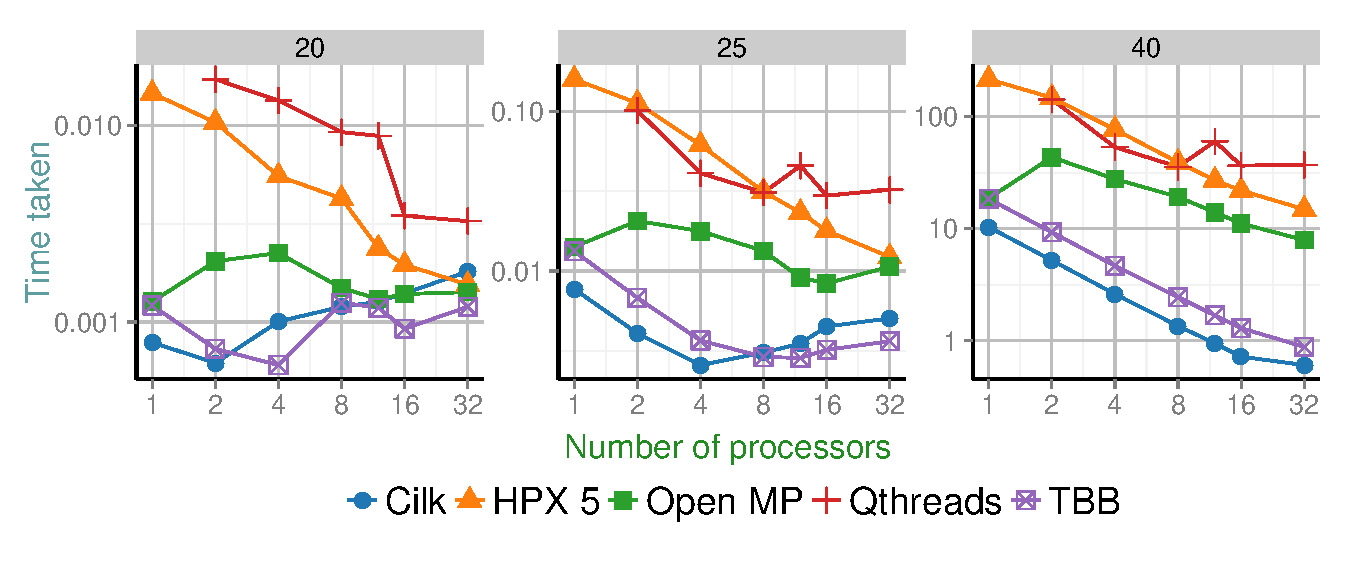
\includegraphics[scale=0.8]{cutter/plots/fib}
\caption{Fibonacci}
\label{fig:fib}
\end{figure}

\begin{figure}[!ht]
\centering
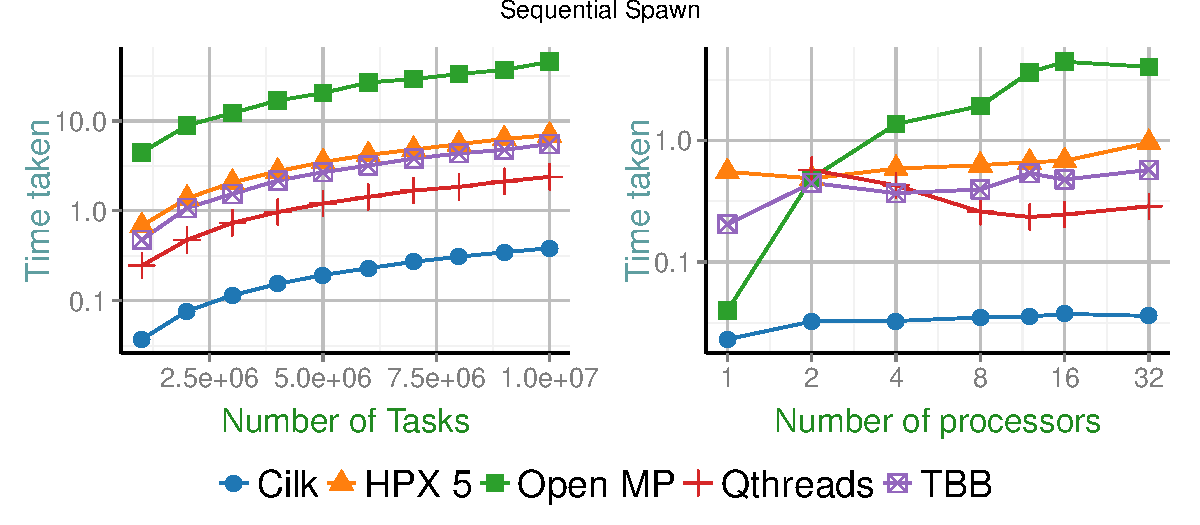
\includegraphics[scale=0.8]{cutter/plots/seq}
\caption{Sequential Spawn}
\label{fig:seq}
\end{figure}

\begin{figure}[!ht]
\centering
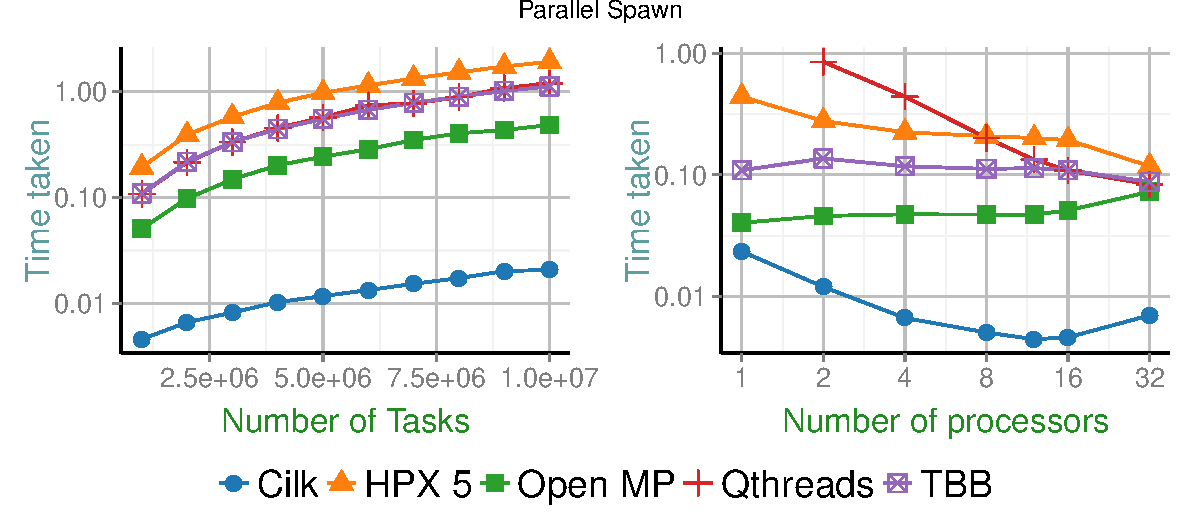
\includegraphics[scale=0.8]{cutter/plots/par}
\caption{Parallel Spawn}
\label{fig:par}
\end{figure}

\end{document}
